\chapter{基于演化博弈的理性隐私风险访问控制模型}
\label{chap:evolutionary-rabac}

\textit{ }

\textit{以数据为中心的大规模用户系统中,现有基于理性的访问控制模型难以满足适应性保护隐私的需求,且博弈参与者的完全理性假设太强,不符合实际场景。针对此问题,本章提出一种面向隐私保护的多参与者理性风险自适应访问控制模型,包含了新的隐私风险量化模块和演化博弈决策模块。首先,基于信息量对访问请求的数据集隐私信息量进行量化,构造了访问请求隐私风险函数和用户隐私风险函数;其次,基于演化博弈在有限理性假设下构建多参与者的访问控制演化博弈模型,利用复制动态方程分析了访问控制参与者的动态策略选择和演化稳定状态形成机理,提出了隐私风险访问控制博弈演化稳定策略的选取方法。仿真实验和对比表明,所提出的访问控制模型能够有效动态自适应地保护敏感信息资源系统中的隐私信息,具有更好的隐私风险适应性,有限理性参与者的动态演化访问策略选取更加符合实际场景。本章成果已投稿至《通信学报》。}

\section{概述}
访问控制是信息系统保障数据安全和系统安全的重要和基础性工具\cite{sandhu1994access}。云计算、大数据及物联网的兴起和发展,使得网络和系统更加复杂、开放,数据安全和隐私需求更加多样化,用户和系统的角色、属性更加难以发掘,需要更加动态化、自适应、细粒度的访问控制模型以满足新环境下的安全和隐私需求\cite{li2017access}。

强制访问控制\cite{mccune2006shamon}、自主访问控制\cite{downs1985issues}、基于角色访问控制\cite{sandhu1996role}等访问控制模型的访问策略是静态的、访问控制粒度粗放,且面对大规模用户的开放系统,难以预先指定用户身份,故这些模型难以适用云计算、大数据和物联网中的新型应用场景。基于属性访问控制\cite{wang2010hierarchical}因其访问控制粒度较细、不需要指定用户身份或角色而受到的广泛的关注,在云计算场景、物联网等得到了广泛的应用,但其需要预先定义访问策略,属性挖掘与属性撤销的计算和实施都比较困难,不能适应动态访问控制需求\cite{servos2017current}。为了解决基于属性访问控制等传统访问控制模型存在的诸多问题,风险和信任被先后引入到访问控制中,提出了基于角色或属性的风险访问控制模型\cite{dimmock2004using,kandala2011attribute,krautsevich2014towards},一定程度上解决了用户访问的动态控制,并进一步发展为基于风险访问控制\cite{cheng2007fuzzy,ni2010risk},更加适用于大数据环境的访问控制需求。同时,医疗、社交网络和位置信息服务等系统的大量多样性数据集访问有了开放性、动态性和隐私敏感需求,隐私侵犯来自内部和外部访问\cite{boulares2017insider},迫切需要能对用户隐私信息在访问过程中进行隐私保护。

访问控制模型中存在授权不足或过度授权的现象,引发数据和系统安全、隐私泄露的风险,亟需能够平衡安全隐私与授权度间的解决方案。访问控制可看做访问主体(用户)与访问客体(服务提供者或系统)间的冲突与合作。博弈论\cite{owen2001game}作为一种解决参与者对抗与合作,并使得参与者获取最大化利益的数学工具,被自然引入到访问控制以平衡安全和访问效用\cite{helil2017non,gao2018game,wang2019game},但现有研究多集中于二人访问控制博弈,要求参与者是完全理性的,难以客观描述访问控制模型中多个用户与系统间的博弈。

本章针对现有访问控制模型难以满足适应性保护隐私的需求,且其访问控制博弈模型难以刻画多用户与系统间的非完全理性对抗与合作问题,基于用户访问隐私风险量化和多人演化博弈,面向开放环境的数据存储隐私保护,提出一种基于演化博弈的多参与者的理性风险访问控制模型,并分析其演化稳定状态和演化稳定策略求解。该访问控制模型在保持风险访问控制优势的同时,通过用户访问隐私风险约束,限制用户高隐私风险的恶意、好奇访问请求,实现隐私保护,同时仅假设参与者有限理性,用多人非合作博弈对多用户对系统资源访问的策略、收益进行分析,通过演化达到博弈演化稳定状态实现了用户和系统间的均衡及稳定,有效平衡隐私保护和访问效用,更加符合现实场景中用户与系统间的策略动态变化选取特征。具体而言,本章的贡献如下:
\begin{enumerate}
	\item 面向开放环境的数据共享隐私保护,在有限理性假设下,通过分析多用户场景的敏感数据隐私保护访问控制问题及需求,提出了一种包含隐私风险量化和演化博弈模块的多人隐私风险自适应访问控制模型。减弱了现有理性访问控制模型的参与者完全理性假设,将二人博弈扩展为多人的群体博弈,且能够适应以数据为中心的系统敏感数据隐私保护需求。
	\item 在“Need-to-Know”的原则下,根据用户访问请求敏感资源的特征,定义了基于信息量化的访问请求隐私风险和用户隐私风险,并给出了自适应的动态隐私风险计算方法。
	\item 对所提出的多用户隐私保护访问控制模型构建了演化博弈模型,提出了基于隐私风险自适应的效用函数,并利用动态复制方程分析并求解了所提出的访问控制模型的博弈演化均衡策略。
	\item 利用动力学理论对所提出的访问控制模型的演化博弈过程进行了仿真,结果表明所提出的多用户隐私风险自适应访问控制模型可在有限理性的演化博弈过程中达到演化稳定状态,能够实现自适应风险的敏感数据隐私保护。
	\item 与相关基于风险访问控制模型和理性访问控制模型相比,分析表明所提出的访问控制模型在以数据为中心的信息系统隐私保护方面具有更好的优势,风险自适应程度好、访问控制参与者假设更符合实际、能达到较好的隐私保护效果。
\end{enumerate}



\section{相关工作}

在风险访问控制\cite{mcgraw2009risk}的概念提出后,Cheng等\cite{cheng2007fuzzy}用多层安全的思路量化了风险,将风险划分为不同等级,实现了该模型的一个实例,但该量化方法缺乏数学理论支持;随后,Ni等\cite{ni2010risk}用模糊推测理论在Cheng等的基础上重新量化风险,使得风险量化满足合取、析取及取反操作需求,用以处置访问访问控制中的紧急访问需求。但文献\cite{cheng2007fuzzy,ni2010risk}中风险量化是静态的,因无法应对访问需求多样、无法预先定义安全等级而缺乏适用性,同时不能满足系统的隐私保护需求,也不能对访问主体的高风险访问进行激励约束。

针对文献\cite{cheng2007fuzzy,ni2010risk}的风险量化静态、不适应高敏感环境问题,Shaikh等\cite{shaikh2012dynamic}利用历史访问行为进行风险和信任动态量化,其风险通过威胁概率和数据泄露影响量化,利用指数移动加权平均算法提出了动态风险的访问控制,以保护系统安全。Armando等\cite{armando2015balancing}参照基于策略访问控制,将访问风险和用户信任进行对比,通过增强用户信任、削减访问安全风险以平衡二者,保护系统资源安全。Diaz-Lopez等\cite{diaz-lopez2016dynamic}将访问风险量化多层分类,并定义对应的风险控制策略,利用遗传算法为动态访问的访问行为提供安全应对措施,以保护高敏感环境的数据安全。但这些方法在风险量化过程中所依赖的信息过多,在实际环境中不能全部获取,易使风险量化不精确而导致访问控制失败。为此,dos Santos等\cite{santos2016framework}提出基于权重的多因子聚合风险量化,并提出一种面向云安全的风险访问控制框架。但文献\cite{shaikh2012dynamic,armando2015balancing,diaz-lopez2016dynamic,santos2016framework}所提出的方法因风险量化是面向安全的,不适用于隐私保护需求。

为了隐私保护需求,Wang等\cite{wang2011quantified}针对医疗信息系统,利用信息熵按照“需要知道”的原则,通过对恶意医生和诚实医生间访问信息的不同,对医生访问病患信息的风险进行量化,提出了一种灵活的风险访问控制模型,但该模型预先假定了诚实医生的行为,风险量化缺乏适应性以对应访问需求变化。在文献\cite{wang2011quantified}的基础上,惠榛等\cite{hui2015risk}利用EM二分算法对基于信息熵的医生访问行为进行区分,监测和控制隐私侵犯的高风险访问性。Zhang等\cite{zhang2018privacy}定义了隐蔽非诚实医生行为,基于时间盒和迭代实现了以主题建模为核心的风险自适应访问控制模型。文献\cite{wang2011quantified,hui2015risk,zhang2018privacy}所提出的方法仅适用于医疗信息系统隐私保护,且并未考虑访问主体与客体间的合作与对抗。针对用户匿名保护需求,Armando等\cite{armando2015risk}将风险访问控制与匿名访问结合,同时考量匿名与数据效用,在匿名系统中抑制高风险访问。本章第\ref{chap:RaBAC-for-privacy}章利用马尔科夫模型对主体访问行为的风险进行量化,并提出了基于信用卡额度约束的风险访问控制模型,在云环境数据隐私保护中激励低风险访问行为,约束高风险访问行为。

与传统访问控制模型中的参与者博弈\cite{gao2018game,hu2014game,liu2016dynamic}类似,基于风险访问控制中的访问主体与客体间也存在二人或多人冲突与合作关系。Helil等\cite{helil2017non}基于二人非合作博弈模型,利用用户信任和访问风险刻画效用函数,分析了风险访问控制模型中的子博弈完美Nash均衡,有效的保证了访问控制决策的科学性,其并未考虑多访问主体访问客体间的冲突与合作。

本章针对开放、动态的大规模多样性数据访问隐私保护需求及多用户与系统间的冲突与合作关系,提出一种多参与者的理性隐私风险自适应访问控制模型。相比于已有工作,该模型仅要求参与者有限理性,通过对访问控制过程中的多参与者的行为、策略和隐私效用的博弈要素进行多参与者演化博弈建模,解决了现有文献对风险访问控制参与者行为刻画不足的问题;通过对历史访问行为和资源建模,利用信息论对访问请求和用户的隐私侵犯风险量进行评估,仅用少量先验信息资源,减少了对系统历史访问信息的要求;仅利用隐私风险量化,不再依赖信任机制,简化了模型的设计复杂度;通过多人演化博弈的演化稳定策略状态求解,不但有效约束了高隐私风险的访问请求,激励用户进行低隐私侵犯访问,且实现了动态风险访问控制的优化访问决策,可有效保护系统隐私数据。

\section{问题描述与建模}
本节首先分析本章所构建的多参与者博弈的风险访问控制模型所要解决的问题,其次提出多参与者隐私风险访问控制模型。

\subsection{多参与者隐私风险访问控制问题描述}
\label{subsec:issues}
在医疗信息系统、情报信息系统、外包计算数据池等环境中存在大量包含个人隐私信息数据,访问的用户量大,且用户不断动态更新访问需求,用户的角色、属性、访问策略等信息难以预先定义,用户为完成其职责不断动态变化访问请求,这些信息难以随用户的访问而动态更新。为了保护隐私信息,需对访问请求的数据所包含的隐私量进行量化,现有的风险访问控制模型难以对隐私进行有效描述和精确动态的量化。访问控制模型中,参与者间是长期的多次访问控制交互,在访问过程中往往无法对所有背景知识和他人的信息全部了解,也无法在每次访问时理性地做出最佳的策略选择,但参与者可模仿其他参与者的高收益策略,调整其后续行为策略,但对非完全理性的多参与者间的冲突与合作博弈行为进行描述极为困难,如何设计激励相容的机制使得参与者诚实合作,尽可能不侵犯隐私,且取得高收益,并使参与者短期利益和长期利益一致。非理性参与者的多人扩展式动态博弈是一个复杂的博弈模型,均衡的存在性证明和求解都极为困难,通过多次交互式博弈和参与者自发策略调整可使博弈逐步处于一种相对稳定状态,即用户稳定地请求低隐私风险访问,即使偶有高隐私风险访问,也会后续调整为低隐私风险访问策略,系统稳定地授权用户低隐私风险访问,即使偶有拒绝授权此类访问,也会后续调整授权策略。
在所提出面向隐私保护的多参与者理性风险访问控制模型中,试图通过以下措施解决上述问题。
\begin{enumerate}
	\item 定义并量化访问请求的隐私风险。依据“Need to Know”的原则,用户为完成工作职责而访问到信息资源中的敏感信息不应当是隐私侵犯,除此之外的访问应当认为是隐私侵犯。在经认证的用户群体中,用户会优先完成自己的职责,其大多数访问请求都是为了完成自己的职责,则该用户单次访问请求与其历史访问请求产生偏移距离,偏离的越远,其违背“Need to Know”原则越严重,访问的隐私信息资源的隐私量越大,隐私风险越高。
	\item 定义并量化用户的隐私风险。将具有相似访问请求行为模式的用户群看作具有相同职责的用户,在历史访问过程中,某一用户的访问偏离该用户群的距离越远,其违背“Need to Know”原则越严重,其用户隐私风险越高;此外,其用户隐私风险直接受其历史访问行为影响,单次的高隐私风险访问将使用户隐私风险提高很快,而单次的低风险访问对用户隐私风险的降低影响较小
	\item 构建演化博弈以刻画多用户和系统的非理性多次博弈。不再对参与者进行绝对理性的假设,而将所有用户和系统视为有限理性的参与者。将访问控制系统的所有参与者看作用户群体和信息资源系统群体,两个群体之间进行多次动态的博弈。博弈过程中,群体中的低收益者会模仿高收益参与者的博弈选择策略,不断进行演化,最终达到稳定的状态,该状态下的参与者策略选择即为演化稳定策略,是参与者的最优策略。
	\item 对(3)中博弈模型设计激励相容的机制。在博弈模型中,对用户的激励主要是通过效用函数的设计来实现。本章对用户的效用函数设计,通过隐私风险量化来计算访问请求的隐私风险和用户隐私风险,分别兼顾短期利益和长期利益。效用函数受到这两个变量的影响,使得对用户而言,长期诚实地访问能使其获得更高的收益,短期的恶意访问虽然能有额外的获得,但却远低于长期收益。同时通过惩罚机制,对短期恶意访问的隐私侵犯行为进行惩罚。促使用户能长期诚实地访问系统。同时,在尽可能吸引更多用户访问系统,亦可阻止恶意的隐私侵犯访问请求的利益促使下,使薪资资源系统能够更加精确、动态地做出有效的策略选择,授权诚实的正常访问,拒绝侵犯隐私的恶意访问。
	\item 对(3)中的博弈模型求解。利用动态复制方程在动力学原理下,分析所提出风险自适应访问控制演化博弈模型的参与者收益函数和信念函数,进一步分析其演化稳定状态及其机理,提出演化稳定策略的求解公式。在不同的初始状态下,通过博弈的不断演化,访问控制博弈总能达到某个演化稳定状态,该状态下的博弈策略选择即为参与者的最优策略。
\end{enumerate}

\subsection{多参与者隐私风险访问控制模型构建}
面向隐私保护需求,多用户和信息资源系统间的有限理性参与者隐私风险访问控制模型如图~\ref{fig:Evolutionary-game-Rabac}所示,包含访问请求决策管理模块、演化博弈建模模块、隐私风险评估模块、上下文信息模块和风险策略模块。

\begin{figure}[htbp]
	\centering
	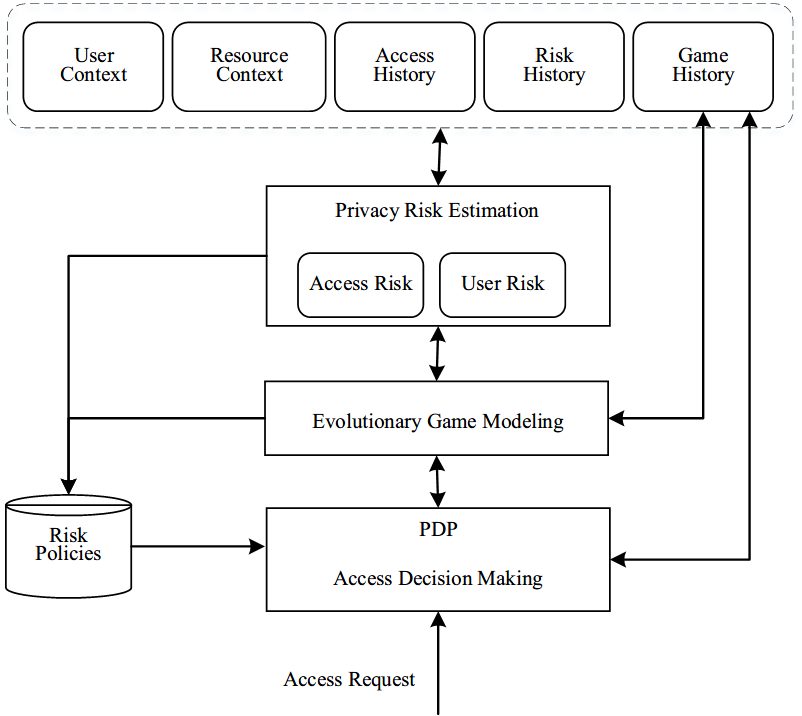
\includegraphics[width = 0.6\linewidth]{./figures/Evolutionary-game-Rabac.png}
	\caption{基于演化博弈的隐私风险访问控制模型}
	\label{fig:Evolutionary-game-Rabac}
\end{figure}

图~\ref{fig:Evolutionary-game-Rabac}中,访问请求决策管理模块接收用户访问请求,根据博弈结果和风险策略模块提供的信息做出授权或不授权等访问决策,并反馈至上下文信息模块;演化博弈建模模块对参与访问控制的用户和系统进行博弈演化,博弈过程中通过隐私风险信息和上下文信息进行动态策略选择,并给出演化策略结果,并将结果反馈给上下文信息模块和访问请求决策管理模块;隐私风险量化模块对访问请求隐私风险和用户隐私风险进行动态量化,支撑演化博弈建模和风险策略更新,并将结果反馈存储至上下文信息模块中;上下文信息模块动态记录并存储用户、信息资源、访问历史、历史隐私风险值、历史博弈策略及收益函数等信息;风险策略池动态更新各用户的隐私风险访问控制策略。

\section{隐私风险定义及自适应计算方法}
本节针对第~\ref{subsec:issues}节所述隐私风险量化问题,分别定义访问请求隐私风险和用户隐私风险,并给出自适应风险计算方法。
\subsection{访问请求隐私风险}

访问控制系统中,信息资源可以通过自然语言处理或机器学习的方式进行标注化,使得所有信息资源记录或原子集合都包含和系统资源使用功能、目的相关的标签信息,如医疗系统中所有的医疗数据可以根据ICD-10标准进行标签化处理,情报系统中所有的情报信息可按照情报属性和功能进行标签化标注。将访问控制过程按照时间划分为不同的时间段${{T}_{0}},{{T}_{1}},{{T}_{2}},\cdots $,每个时间段是一小时、一天或一周等。用户U在前一个时间段T内和当前时间段截止目前向系统发出了$n$次访问请求$q_{1}^{U},q_{2}^{U},\cdots ,q_{n}^{U}$,对应的访问信息资源集合(实际应用中利用信息资源集合对应的标签集合进行风险计算)为$R_{1}^{U},R_{2}^{U},$ $\cdots ,R_{n}^{U}$,则U访问的信息资源集合为$R_{{}}^{U}\text{=}\bigcup\nolimits_{i=1}^{n}{R_{i}^{U}}$。当前用户$U$的访问请求为$q_{0}^{U}$,该请求对应的系统信息资源集合为$R_{0}^{U}$。根据各用户的历史访问信息资源集合的相似性和聚类,可将具有相似访问行为的用户划分为一组,在某一组中,所有的用户具有相同的系统职责,在访问行为上仅有较小的差异。设用户$U$属于用户分类组$g$,用户分类组$g$在前一个时间段T内和当前时间段截止目前,访问的信息资源集合为$R_{{}}^{g}$。则用户$U$的当前访问请求$q_{0}^{U}$隐私风险为

\begin{equation}
r(q_{0}^{U})=\begin{cases}
1, & \text{ 若 } R_{0}^{U}/{{R}^{g}}\ne \varnothing \\ 
\alpha \frac{-|R_{0}^{U}/{R}^{U}|max_{x\in R_{0}^{U}/{R}^{U}}logp(x)}{-\sum_{x\in{R^U}}logp(x)}+ \beta \frac{-\sum_{x\in R_0^U \cap  R^U}logp(x)}{-\sum_{x\in  R^U}logp(x)}& \text{若 } R_{0}^{U}/{{R}^{g}}=\varnothing 
\end{cases}
\end{equation}
其中$p(x)$表示x在$R_{{}}^{g}$中的概率,$1>\alpha >\beta >0$,且$\alpha \text{+}\beta \text{=}1$。
根据用户组$g$中用户的访问请求风险值的历史及分布可利用分位数设置阈值${{t}_{g}}$,若$r(q_{0}^{U})>{{t}_{g}}$,则定义$q_{0}^{U}$为隐私侵犯访问请求,否则其为非隐私侵犯访问请求。特别注意的是,前述定义是从系统的角度看待某一访问请求,用户$U$会主动选择正常访问或隐私侵犯访问,但系统仅根据访问请求本身来判定,可能将用户的正常访问识别为隐私侵犯访问,亦有可能将用户的隐私侵犯访问识别为非隐私侵犯访问。当将某一访问请求为识别为隐私侵犯访问时,用户可通过风险消除措施降低隐私风险,文献\cite{diaz-lopez2016dynamic}讨论了相关措施。

\subsection{用户隐私风险}
用户$U$的隐私风险是根据其访问行为特征而发生变化,当用户访问请求隐私风险值高,则用户的隐私风险提高,用户访问请求隐私风险值低,则用户隐私风险降低,且用户隐私风险提高的速率高而降低的速率低。这样的假设与银行对客户的信用风险评估一致,若客户发生一次信用违约,其信用风险提高很快,而需要很多次的信用守约才能将其信用风险降低至原来的值。用户隐私风险仅与其前一隐私风险值和前一次访问请求隐私风险值相关。设用户U的初始隐私风险值为$r_{0}^{U}$,其在当前访问请求$q_{0}^{U}$之前的隐私风险值为$r_{n}^{U}$,则当前访问请求$q_{0}^{U}$发出之后,系统根据其隐私风险值$r_{n}^{U}$和访问请求$q_{0}^{U}$的隐私风险值$r(q_{0}^{U})$计算用户$U$的更新隐私风险值

\begin{equation}\label{eq:users-risk}
r_{n+1}^{U}=\begin{cases}
r_{n}^{U}+r(q_0^U), & \text{ 若 } q_0^U) \text{是一个隐私侵犯访问请求}; \\ 
r_{n}^{U}-r(q_0^U),& \text{反之}
\end{cases}
\end{equation} 
由于当$q_{0}^{U}$是隐私侵犯访问请求时,其隐私风险值要大于当$q_{0}^{U}$是非隐私侵犯访问请求时的隐私风险值,故公式~\ref{eq:users-risk}中用户U的隐私风险值$r_{n+1}^{U}$符合增长快,下降慢的特征。

\section{所提出访问控制模型的演化博弈模型及均衡分析}
\label{sec:evolutionary-game-model}
本节将访问敏感信息的用户和信息资源系统看作两个有限理性的群体,两个群体中的参与者进行动态演化博弈,通过不断演化达到演化稳定状态,所有博弈参与者都选取到最优博弈策略。定义隐私风险访问控制的演化博弈模型,包含参与者、博弈策略、信念和收益函数,并给出演化稳定策略均衡求解计算方法,进一步分析演化稳定状态及演化稳定策略的特征和机理。

\subsection{隐私风险访问控制的演化博弈模型}
\label{subsec:evolutionary-game-model}
在有限理性参与者假设下,基于演化博弈可构建面向隐私保护的风险自适应访问控制演化博弈模型。
\begin{definition}
	风险自适应访问控制演化博弈模型(Risk-adaptive based access control evolutionary game model),可表示为4元组$RaBACEGM=(P,A,\Pr ,u)$。
	\begin{enumerate}
		\item $P=\{U,S\}$是演化博弈的参与者空间,其中$U$是用户,$S$是信息资源系统。
		\item $A=\{{{A}_{U}},{{A}_{S}}\}$是博弈策略空间,其中${{A}_{U}}=$ $\{Normal,Malicious\}$是用户的可选策略集合,包含正常访问和恶意访问两种,${{A}_{S}}=\{Grant,Deny\}$是信息资源系统的可选策略集合,包含授权和拒绝两种。
		\item $\Pr =\{p,q\}$是博弈信念集合,其中$p=\{{{p}_{Normal}},{{p}_{Malicious}}\}$表示用户分别采取正常访问和恶意访问的概率,且${{p}_{Normal}}\text{+}{{p}_{Malicious}}=1$;$q=\{{{q}_{Grant}},$ ${{q}_{Deny}}\}$表示信息资源系统分别采取授权和拒绝的概率,且${{q}_{Grant}}+{{q}_{Deny}}=1$。
		\item $u=\{{{u}_{U}},{{u}_{S}}\}$是博弈参与者的收益函数集合,其中${{u}_{U}}\text{= }\!\!\{\!\!\text{ }u_{U}^{N,G}\text{,}u_{U}^{N,D},u_{U}^{M,G},u_{U}^{M,D}\text{ }\!\!\}\!\!\text{ }$是用户的收益函数,${{u}_{S}}\text{= }\!\!\{\!\!\text{ }u_{S}^{N,G}\text{,}u_{S}^{N,D},u_{S}^{M,G},u_{S}^{M,D}\text{ }\!\!\}\!\!\text{ }$是信息资源系统的收益函数,二者的值由参与者的访问策略选择所决定。
		
	\end{enumerate}
\end{definition}

本章的访问控制系统中,用户$U$和资源信息系统$S$都有两个策略可以选择,在博弈的不同阶段,用户和资源信息系统对策略的选择概率不同,且该概率根据演化博弈的演化学习机制而不断变化,使得访问控制参与者的策略选择形成动态变化的过程。该博弈模型形成的基本博弈树如图\ref{fig:game-tree}所示,表示单次博弈中用户与信息资源系统的博弈策略和收益情况。

\begin{figure}[htbp]
	\centering
	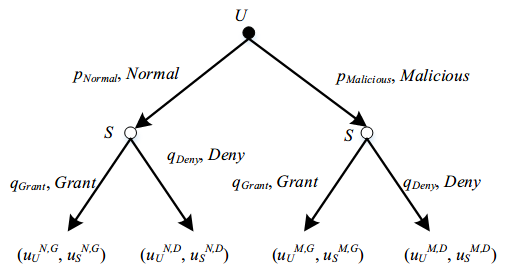
\includegraphics[width = 0.6\linewidth]{./figures/game-tree.png}
	\caption{风险自适应访问控制演化博弈模型的基本博弈树}
	\label{fig:game-tree}
\end{figure}

博弈参与者根据自身和其他参与者的策略选择而获取不同的数值收益,所有参与者的收益矩阵如表\ref{tab:privacy-utilities-matrix}所示。

\begin{table}[htbp]
	\caption{风险自适应访问控制演化博弈模型的基本收益矩阵}
	\label{tab:privacy-utilities-matrix}
	\centering
	\begin{tabular}{cccc}%
		
		\toprule
		\textbf{ }&\textbf{ }&\multicolumn{2}{c}{信息资源系统$S$}\\
		\textbf{ }&\textbf{ }& $q_{Grant}$,$Grant$&$q_{Deny}$,$Deny$\\
		\midrule
		\multirow{2}{*}{用户$U$} & $p_{Normal}$,$Normal$ &$u_U^{N,G}$, $u_S^{N,G}$ & $u_U^{N,D}$, $u_S^{N,D}$\\
		& $p_{Malicious}$,$Malicious$ &$u_U^{M,G}$, $u_S^{M,G}$ & $u_U^{M,D}$, $u_S^{M,D}$\\
		\bottomrule
	\end{tabular}
\end{table}

表\ref{tab:privacy-utilities-matrix}中对演化博弈模型中各参与者的信念、策略和收益进行了形式化描述,特别的,参与者的收益根据访问请求的隐私风险不同而不同。


\begin{enumerate}
	\item  $u_{U}^{N,G}>0$表示用户采用正常访问策略,被授权访问时的收益。该收益由正常访问获取工作职责完成的信息价值决定,并受到用户的隐私风险影响,用户的隐私风险越低其收益越高,反之越低,可表示为$u_{U}^{N,G}=U_{Benefit}^{N,G}(r_{\max }^{U}-{{r}^{U}})$,其中$U_{Benefit}^{N,G}$为用户采用正常访问策略被授权访问时的基础性收益,$r_{\max }^{U}$为用户的最大隐私风险,${{r}^{U}}$为用户的当前隐私风险。
	\item  $u_{U}^{N,D}=0$表示用户采用正常访问策略,被拒绝访问时的收益,该值为0。
	\item  $u_{U}^{M,G}>0$表示用户采用恶意访问策略,进行隐私侵犯访问被授权访问时的收益。该收益由用户正常访问的收益、隐私侵犯访问的额外收益组成,并受用户的隐私风险和当前访问请求的隐私风险影响。收益表示为$u_{U}^{M,G}=U_{Benefit}^{N,G}(r_{\max }^{U}-{{r}^{U}})+U_{Extra}^{M,G}\cdot (r_{\max }^{U}-{{r}^{U}})\cdot r({{q}^{U}})$,其中$U_{Extra}^{M,G}$为用户采用恶意访问策略被授权访问时的基础性额外收益。
	\item  $u_{U}^{M,D}<0$表示用户采用恶意访问策略,进行隐私侵犯访问被拒绝访问时的收益。该收益是信息资源系统对用户的惩罚,并受到用户隐私风险和访问请求隐私风险的影响,风险值越大惩罚越大。该收益表示为$u_{U}^{M,D}\text{=}U_{Punish}^{M,D}\cdot {{r}^{U}}\cdot r({{q}^{U}})$,其中$U_{Punish}^{M,G}$是对用户在采取恶意访问策略时的基础性惩罚。
	\item  $u_{S}^{N,G}>0$表示信息资源系统授权用户正常的访问请求时的收益。该收益是用户正常访问时完成工作职责时对系统的正向回馈,并受用户的隐私风险影响,用户隐私风险越低,系统收益越大。该收益可表示为$u_{S}^{N,G}\text{=}S_{Benefit}^{N,G}(r_{\max }^{U}-{{r}^{U}})$,其中$S_{Benefit}^{N,G}$为系统得到的基础性正向回馈。
	\item $u_{S}^{N,D}<0$表示信息资源系统拒绝用户正常的访问请求时的收益。该收益是信息资源系统拒绝用户正常访问,无法完成用户工作职责而对系统造成的损失,用户的隐私风险越低,对系统的损失越大。该收益可表示为$u_{S}^{N,D}\text{=}S_{Loss}^{N,D}(r_{\max }^{U}-{{r}^{U}})$,其中$S_{Loss}^{N,D}$为系统受到的基础性损失。
	\item  $u_{S}^{M,G}<0$表示信息资源系统授权用户恶意访问请求时的收益。该收益是被用户恶意访问所损失的隐私信息价值,受用户访问请求的隐私风险和用户隐私风险,风险值越大,信息资源系统的损失越大。该收益可表示为$u_{S}^{M,G}\text{=}S_{Loss}^{M,G}\cdot {{r}^{U}}\cdot r({{q}^{U}})$,其中$S_{Loss}^{M,G}$表示信息资源系统授权用户恶意访问时的基础性损失。
	\item $u_{S}^{M,D}=0$表示信息资源系统拒绝用户的恶意访问时的收益。
\end{enumerate}

基于表\ref{tab:privacy-utilities-matrix}可计算用户不同访问策略的期望收益和平均收益为
\begin{eqnarray}\label{eq:utilities-users}
u_{U}^{Normal}={{q}_{Grant}}u_{U}^{N,G}+{{q}_{Deny}}u_{U}^{N,D} \\ 
 u_{U}^{Malicious}={{q}_{Grant}}u_{U}^{M,G}+{{q}_{Deny}}u_{U}^{M,D} \\ 
{{\overline{u}}_{U}}={{p}_{Normal}}u_{U}^{Normal}+{{p}_{Malicious}}u_{U}^{Malic\text{i}ious}
\end{eqnarray}


由于风险访问收益较低者会学习模仿高收益者所选取的策略,针对用户可选策略集合${{A}_{U}}=\{Normal,Malicious\}$,选取不同策略的用户比例将随时间而发生变化,用${{p}_{Normal}}(t)$表示选取正常访问策略的用户比例,${{p}_{Malicious}}(t)$表示选取正常访问策略的用户比例,满足${{p}_{Normal}}(t)\text{+}{{p}_{Malicious}}(t)\text{=}1$。对于某一用户访问策略,选取该策略的用户比例是时间的函数,其动态变化速率可用复制动态方程表示。

\begin{equation}\label{eq:dynamic-equantion1}
D({{p}_{i}})=\frac{d{{p}_{i}}(t)}{dt}=p(u_{U}^{i}-{{\overline{u}}_{U}})
\end{equation}
其中$i\in \{Normal,Malicious\}$。
同理,信息资源系统不同策略选择的期望收益和平均收益为

\begin{align}
& u_{S}^{Grant}={{p}_{Normal}}u_{S}^{N,G}+{{p}_{Malicious}}u_{S}^{M,G} \\ 
& u_{S}^{Deny}={{p}_{Normal}}u_{S}^{N,D}+{{p}_{Malicious}}u_{S}^{M,D} \\ 
& {{\overline{u}}_{S}}={{q}_{Grant}}u_{S}^{Grant}+{{q}_{Deny}}u_{S}^{Deny} \\ 
\end{align}

对信息资源系统的博弈策略选取亦可建立复制动态方程
\begin{equation}\label{eq:dynamic-equantion2}
A({{q}_{j}})=\frac{d{{q}_{j}}(t)}{dt}=q(u_{S}^{j}-{{\overline{u}}_{S}})
\end{equation}
其中$j\in \{Grant,Deny\}$。通过联立式\ref{eq:dynamic-equantion1}和\ref{eq:dynamic-equantion2},令
\begin{equation}\label{eq:differential-equation}
Y=[ D(p), A(q)]'=f(Y,t)=0
\end{equation}
可求解公式\ref{eq:differential-equation},即可得到隐私风险访问模型的演化博弈平衡状态点,从而实现访问控制策略选取的分析和预测。

\subsection{隐私风险访问控制博弈演化稳定策略均衡求解}
\label{subsec:solution}
所提出的隐私风险访问控制模型中,用户选取不同的访问行为策略会产生不同的收益,收益低的用户会模仿收益高的用户所选取的访问行为策略。对于相同工作职责的$n$个用户,有两种访问策略$\{Normal, Malicious\} $可选,选取这两种访问策略的用户比例随着时间发生变化,分别为$p_{Normal}(t)$和$1-p_{Normal}(t)$。对于访问策略$Normal$,选取该策略的用户人数比例是时间的函数,其动态变化速率可表示为动态复制函数

\begin{equation}\label{eq:dynamic-equations}
D({{p}_{Normal}})=\frac{d{{p}_{Normal}}(t)}{dt}={{p}_{Normal}}(u_{U}^{Normal}-{{\overline{u}}_{U}})
\end{equation}

 令$D({{p}_{Normal}})=0$,将式\ref{eq:utilities-users}代入\ref{eq:dynamic-equations}可求解,得${{p}_{Normal}}=0$,${{p}_{Normal}}\text{=}1$和${{q}_{Grant}}=\\\frac{u_{U}^{M,D}-u_{U}^{M,G}}{u_{U}^{N,G}-u_{U}^{N,D}\text{-}u_{U}^{M,G}\text{+}u_{U}^{M,D}}$。
 
 类似地,信息资源系统的两种可选行为策略$\{Grant,Deny\}$及其策略选取概率$q_{Grant}(t)$~\\和$1-q_{Grant}(t)$,对于策略Grant的选取概率时间变化函数,亦可求解得$q=0$,$q=1$和${{p}_{Normal}}=\frac{u_{S}^{M,D}-u_{S}^{M,G}}{u_{S}^{N,G}-u_{S}^{N,D}\text{-}u_{S}^{M,G}\text{+}u_{S}^{M,D}}$。

将用户与信息资源系统的策略选取复制动态方程相结合,构建隐私风险访问控制演化博弈方程组,对博弈模型进行稳定性分析。求解方程组得5个解 ${{Y}_{1}}=[0,1]'$,${{Y}_{2}}=\left[ 0 ,1 \right]'$,${{Y}_{3}}=\left[1 ,0 \right]'$,${{Y}_{4}}=\left[ 1 ,1 \right]'$和${{Y}_{5}}=
\begin{bmatrix}
\frac{u_{S}^{M,D}-u_{S}^{M,G}}{u_{S}^{N,G}-u_{S}^{N,D}\text{-}u_{S}^{M,G}\text{+}u_{S}^{M,D}},
\frac{u_{U}^{M,D}-u_{U}^{M,G}}{u_{U}^{N,G}-u_{U}^{N,D}\text{-}u_{U}^{M,G}\text{+}u_{U}^{M,D}}
\end{bmatrix}'$。其中,${{Y}_{1}}=[0,1]'$表示用户选取纯策略恶意访问请求$Malicious$,信息资源系统选取纯策略拒绝访问$Deny$;${{Y}_{2}}=\left[ 0 ,1 \right]'$表示用户纯策略选取恶意访问请求$Malicious$,信息资源系统选取纯策略允许访问$Grant$;${{Y}_{3}}=\left[1 ,0 \right]'$表示用户纯策略选取正常访问请求$Normal$,信息资源系统选取纯策略拒绝访问$Deny$;${{Y}_{4}}=\left[ 1 ,1 \right]'$表示用户纯策略选取正常访问请求$Normal$,信息资源系统选取纯策略允许访问$Grant$;${{Y}_{5}}=
\begin{bmatrix}
\frac{u_{S}^{M,D}-u_{S}^{M,G}}{u_{S}^{N,G}-u_{S}^{N,D}\text{-}u_{S}^{M,G}\text{+}u_{S}^{M,D}},
\frac{u_{U}^{M,D}-u_{U}^{M,G}}{u_{U}^{N,G}-u_{U}^{N,D}\text{-}u_{U}^{M,G}\text{+}u_{U}^{M,D}}
\end{bmatrix}'$表示用户以混合概率组合$( \frac{u_{S}^{M,D}-u_{S}^{M,G}}{u_{S}^{N,G}-u_{S}^{N,D}\text{-}u_{S}^{M,G}\text{+}u_{S}^{M,D}}, 1- \frac{u_{S}^{M,D}-u_{S}^{M,G}}{u_{S}^{N,G}-u_{S}^{N,D}\text{-}u_{S}^{M,G}\text{+}u_{S}^{M,D}})$选取策略$\{Normal, Malicious\}$,信息资源系统以混合概率组合$(\frac{u_{S}^{M,D}-u_{S}^{M,G}}{u_{S}^{N,G}-u_{S}^{N,D}\text{-}u_{S}^{M,G}\text{+}u_{S}^{M,D}} , 1-\frac{u_{S}^{M,D}-u_{S}^{M,G}}{u_{S}^{N,G}-u_{S}^{N,D}\text{-}u_{S}^{M,G}\text{+}u_{S}^{M,D}} )$选取策略$\{Grant, Deny\}$。根据演化稳定策略理论可知$Y_1$、$Y_2$、$Y_3$、$Y_4$为鞍点,$Y_5$为中心点,故所提出的风险自适应访问控制演化博弈模型存在演化稳定均衡。

\subsection{隐私风险访问控制博弈演化稳定策略分析}
演化稳定策略是演化博弈模型中能够抵抗侵犯的策略。在所提出的风险自适应访问控制演化博弈模型中,用户和信息资源系统双方各自存在复制动态,以用户为例,对其演化稳定策略进行分析。通过式\ref{eq:dynamic-equations}可知,用户正常访问请求策略选取的复制动态相位有3种,当${{q}_{Grant}}=\frac{u_{U}^{M,D}-u_{U}^{M,G}}{u_{U}^{N,G}-u_{U}^{N,D}\text{-}u_{U}^{M,G}\text{+}u_{U}^{M,D}}$时,对任意的用户正常访问请求$Normal$策略选取概率$p_{Normal}$,有$\frac{d{{p}_{Normal}}(t)}{dt}\text{=0}$,但是一旦$q_{Grant}$的取值发生偏移,$frac{d{{p}_{Normal}}(t)}{dt}$就会剧烈变化,其所代表的状态不具有稳定性;当${{q}_{Grant}}>\frac{u_{U}^{M,D}-u_{U}^{M,G}}{u_{U}^{N,G}-u_{U}^{N,D}\text{-}u_{U}^{M,G}\text{+}u_{U}^{M,D}}$时,$p_{Normal}= 1$为用户的演化稳定策略;当${{q}_{Grant}}<\frac{u_{U}^{M,D}-u_{U}^{M,G}}{u_{U}^{N,G}-u_{U}^{N,D}\text{-}u_{U}^{M,G}\text{+}u_{U}^{M,D}}$时,$p_{Normal}=0$为用户的演化稳定策略。

 同理,信息资源系统授权策略选取的复制动态相位有3种,当${{p}_{Normal}}=\frac{u_{S}^{M,D}-u_{S}^{M,G}}{u_{S}^{N,G}-u_{S}^{N,D}\text{-}u_{S}^{M,G}\text{+}u_{S}^{M,D}}$时,对任意的授权访问策略选取概率$q_{Grant}(t)$,有$\frac{d{{q}_{Grant}}(t)}{dt}\text{=0}$,该状态不具有稳定性;当${{p}_{Normal}}>\frac{u_{S}^{M,D}-u_{S}^{M,G}}{u_{S}^{N,G}-u_{S}^{N,D}\text{-}u_{S}^{M,G}\text{+}u_{S}^{M,D}}$时,$q_{Grant}(t)=1$是信息资源系统的演化稳定策略;当${{p}_{Normal}}<\frac{u_{S}^{M,D}-u_{S}^{M,G}}{u_{S}^{N,G}-u_{S}^{N,D}\text{-}u_{S}^{M,G}\text{+}u_{S}^{M,D}}$时,$q_{Grant}(t)=0$是信息资源系统的演化稳定策略。
 
 
 \section{实验仿真与分析}
本节对本章提出的隐私风险自适应访问控制模型的演化博弈过程,利用动力学理论进行仿真,分析隐私风险自适应访问控制演化博弈模型的最优访问策略选取问题。

 由\ref{subsec:solution}节可知,该访问控制模型的演化博弈稳定状态为${{Y}_{1}}=[0,0]'$,${{Y}_{2}}=[0,1]'$,${{Y}_{3}}=[1,0]'$和${{Y}_{4}}=[1,1]'$,下面针对 和 的不同初始状态,进行实验仿真。通过仿真可以观察出$p_{Normal}$和$q_{Grant}$的演化趋势,得到最终的演化稳定状态,通过演化分析,实现隐私风险访问控制系统中参与者的策略选择预测,从而选取出最优的访问控制策略。本章的仿真实验中,根据\ref{subsec:evolutionary-game-model}节中的分析对用户的效用函数设定为$u_{U}^{N,G}>u_{U}^{M,G}>u_{U}^{N,D}>u_{U}^{M,D}$,对信息资源系统的效用函数设定为$u_{S}^{N,G}>u_{S}^{M,D}>u_{S}^{N,D}>u_{S}^{M,G}$。

\begin{enumerate}
 	\item 当初始状态为${{p}_{Normal}}\text{=0}$,${{q}_{Grant}}\in [0,1)$时,用户以概率1选取恶意访问$Normal$策略,信息资源系统以概率1选取拒绝访问Deny策略或任意其他混合策略选取授权访问$Grant$、拒绝访问$Deny$策略,通过系统仿真,经过演化,用户和信息资源系统双方的策略选取都会演化为${{p}_{Normal}}\text{=0}$,${{q}_{Grant}}=0$的概率,即用户以纯策略选取恶意访问$Malicious$,信息资源系统以纯策略选取拒绝访问$Deny$。${{p}_{Normal}}$和${{q}_{Grant}}$的具体演化曲线如图\ref{fig:Evolutionary-exp1}所示,在达到演化稳定状态${{Y}_{1}}=[0,0]'$时,风险自适应访问控制演化博弈模型的博弈参与者两方博弈策略选取最优。
 	
 	 \begin{figure}[htbp]
 		\centering
 		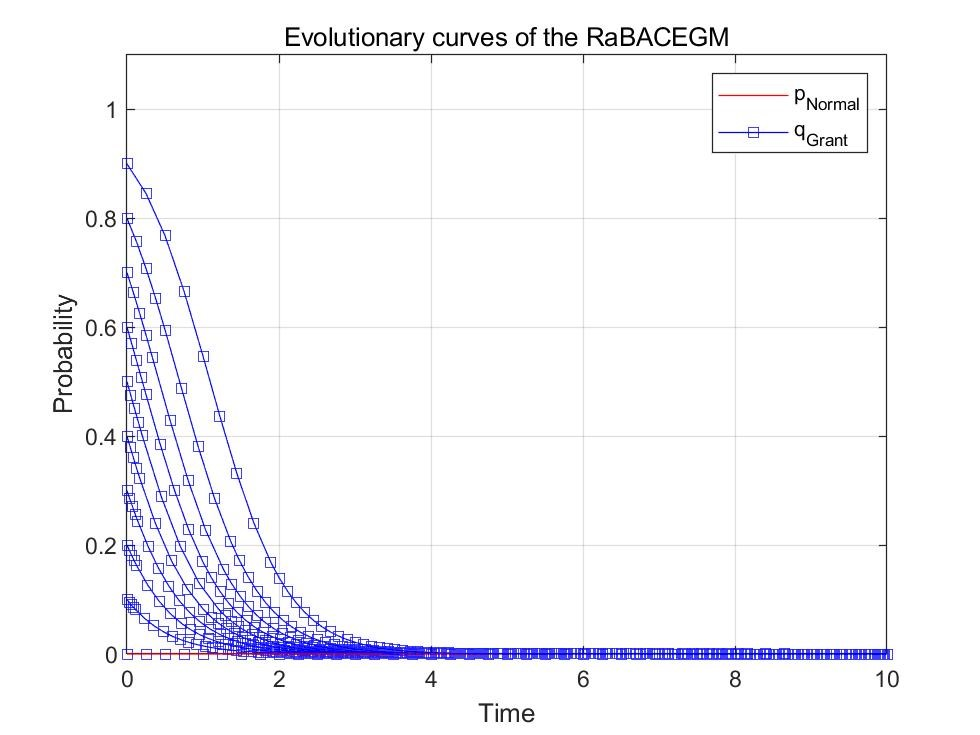
\includegraphics[width=0.8\linewidth]{./figures/Evolutionary-exp1.jpg}
 		\centering
 		\caption{初始状态为$p_{Normal}=0,q_{Grant}∈[1,0)$时,隐私风险自适应访问控制演化博弈模型的演化曲线,演化稳定状态为$p_{Normal}=0, q_{Grant}=0$}\label{fig:Evolutionary-exp1}
 	\end{figure}
 
 	\item 当初始状态为${{p}_{Normal}}\text{=0}$,${{q}_{Grant}}\text{=}1$时,用户以概率1选取恶意访问$Malicious$策略,信息资源系统以概率1选取授权访问$Grant$策略,通过演化,该演化博弈模型的博弈双方的策略选取不变,${{p}_{Normal}}$和${{q}_{Grant}}$的具体演化曲线如图\ref{fig:Evolutionary-exp2}所示。
 	
 	 \begin{figure}[htbp]
 		\centering
 		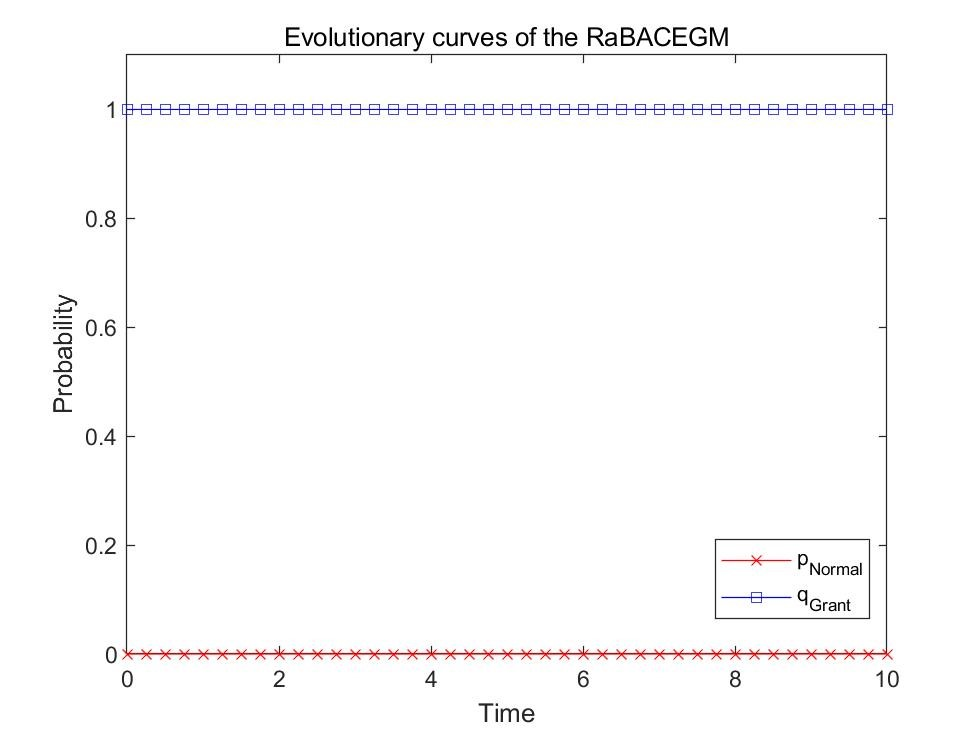
\includegraphics[width=0.8\linewidth]{./figures/Evolutionary-exp2.jpg}
 		\centering
 		\caption{初始状态为时 $p_{Normal}=0,q_{Grant}=1$,隐私风险自适应访问控制演化博弈模型的演化曲线,演化稳定状态为$p_{Normal}=0, q_{Grant}=1$}\label{fig:Evolutionary-exp2}
 	\end{figure}
 
 		在图\ref{fig:Evolutionary-exp2}中,尽管该演化过程的最终状态${{Y}_{2}}=[0,1]'$是所提出的演化博弈模型的演化稳定状态,但在实际应用中,信息资源系统为了遏制恶意访问请求,保护系统中的隐私数据,同时尽可能吸引更多用户访问系统,其不会以纯策略方式选取授权访问$Grant$,故当用户初始访问策略选取为纯策略恶意访问$Malicious$时,会转换为图\ref{fig:Evolutionary-exp1}所示的演化曲线。
 		
 	\item 当初始状态为${{p}_{Normal}}\in (0,1]$,${{q}_{Grant}}\in (0,1]$时,用户以混合策略方式选取正常访问$Normal$、恶意访问$Malicious$,或以纯策略方式(概率为1)选取正常访问$Normal$,信息资源系统以混合策略方式选取授权访问$Grant$、拒绝访问$Deny$,或以纯策略方式(概率为1)选取拒绝访问$Deny$,博弈模型通过不断演化,会达到演化稳定状态${{Y}_{4}}=[1,1]'$,即用户以纯策略方式选取正常访问$Normal$,信息资源系统以混合策略方式选取授权访问$Grant$。该状态下风险自适应访问控制演化博弈模型的博弈策略选择最优,${{p}_{Normal}}$和${{q}_{Grant}}$的演化曲线如图6所示。
 	
 	\begin{figure}[htbp]
 		\centering
 		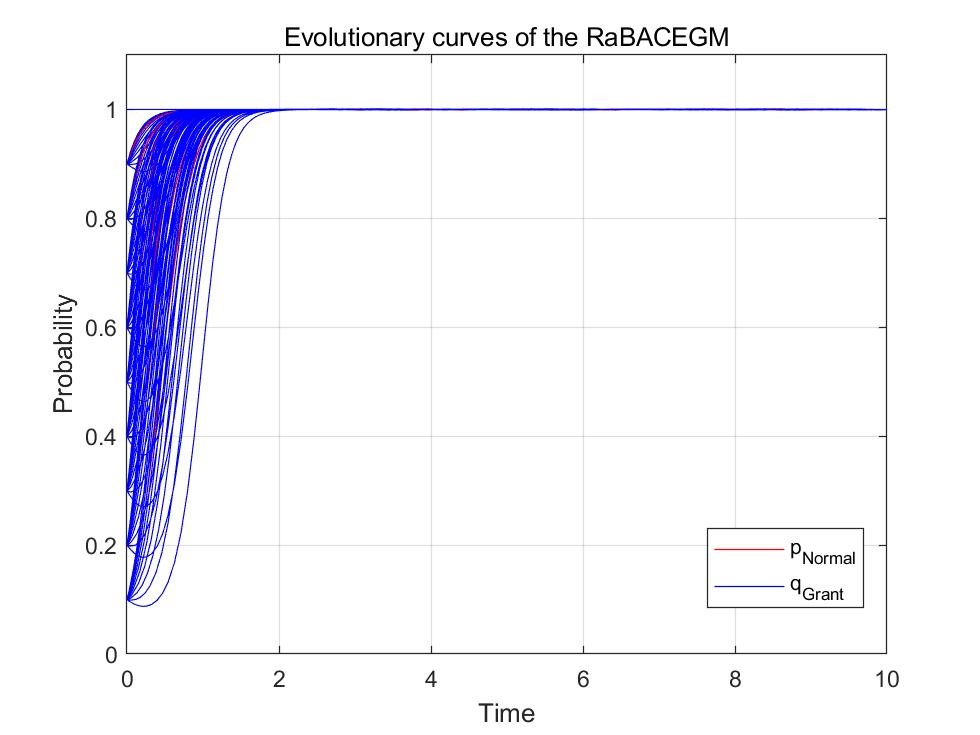
\includegraphics[width=0.8\linewidth]{./figures/Evolutionary-exp3.jpg}
 		\centering
 		\caption{初始状态为$p_{Normal}\in (0,1]$,$q_{Grant}\in (0,1]$时,隐私风险自适应访问控制演化博弈模型的演化曲线,演化稳定状态为$p_{Normal}=1$,$q_{Grant}=1$}\label{fig:Evolutionary-exp3}
 	\end{figure}
 
 	\item 当初始状态为${{p}_{Normal}}\in (0,1]$,${{q}_{Grant}}\text{=}0$时,用户以混合策略方式选取正常访问$Normal$、恶意访问$Malicious$,或以纯策略方式(概率为1)选取正常访问$Normal$,信息资源系统以纯策略方式(概率为1)选取拒绝访问$Deny$,通过不断演化,会达到演化稳定状态${{p}_{Normal}}\text{=}1$,${{q}_{Grant}}\text{=}0$,即用户以纯策略方式选取正常访问$Normal$,信息资源系统以纯策略方式选取拒绝访问$Deny$。${{p}_{Normal}}$和${{q}_{Grant}}$的具体演化曲线如图\ref{fig:Evolutionary-exp4}所示。
 	
 	\begin{figure}[htbp]
 		\centering
 		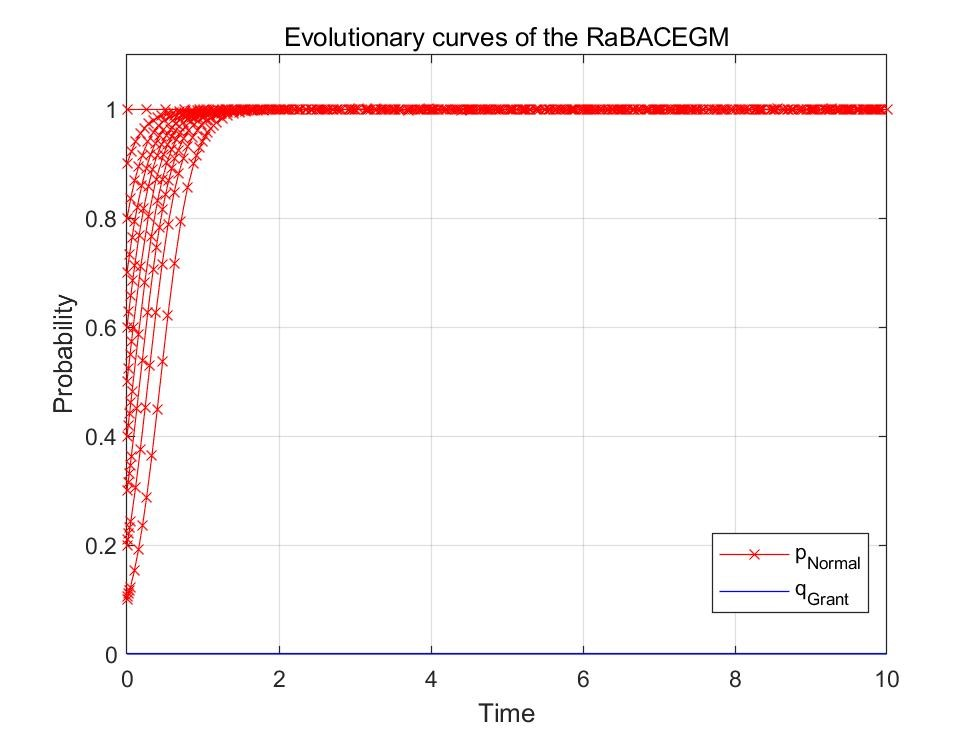
\includegraphics[width=0.8\linewidth]{./figures/Evolutionary-exp4.jpg}
 		\centering
 		\caption{初始状态为$p_{Normal}\in(0,1],q_Grant=0$时,隐私风险自适应访问控制演化博弈模型的演化曲线,演化稳定状态为$p_{Normal}=1,q_{Grant}=0$}\label{fig:Evolutionary-exp4}
 	\end{figure}
 	
 	在图\ref{fig:Evolutionary-exp4}中,最终达到的演化状态是风险自适应访问控制演化博弈模型的演化稳定状态${{Y}_{3}}=[10]'$。但在实际应用中,信息资源系统为了吸引更多用户访问系统,其不会以纯策略方式选取拒绝访问Deny,会以混合策略的方式选取其博弈策略,其演化过程会转换为图\ref{fig:Evolutionary-exp3}所示的演化曲线。
 \end{enumerate}


 由以上仿真结果可知,给定不同的策略选取初始状态,经过演化,所提出的风险自适应访问控制模型在演化博弈过程中会达到某个稳定状态。通过观察对比,本演化博弈模型的模拟演化结果与第\ref{sec:evolutionary-game-model}节中的理论分析保持一致,说明该演化博弈模型与现实系统中的规律相符。因此,本章提出的风险自适应访问控制演化博弈模型具有有效性,可将其应用于面向隐私保护的风险自适应访问控制系统中,为访问控制系统的参与者进行隐私保护访问策略选取提供依据。
 
 \section{对比与讨论}
 
 在风险访问控制、基于博弈的访问控制和基于演化博弈的信息安全模型方面均有相应的研究,本节针对这些研究工作进行对比,如表\ref{tab:game-model-comparision}所示。
\begin{table}[htbp]
	\caption{所提出风险自适应访问控制模型的对比}
	\label{tab:game-model-comparision}
	\centering
	\begin{tabular}{ccccc}%
		
		\toprule
		文献  &	访问控制目的&	风险量化&	博弈参与者&	博弈方法\\
		\midrule
		文献\cite{ni2010risk}&
		安全保护&	静态安全风险量化&	-&	-\\
		文献\cite{shaikh2012dynamic}&
		安全保护&	风险和信任动态量化&	-&	-\\
		文献\cite{santos2016framework}&
		云安全保护&	多因子聚合风险量化&	-&	-\\
		文献\cite{wang2011quantified}&
		医疗信息隐私保护&	静态隐私风险量化&	-&	-\\
		文献\cite{zhang2018privacy}&
		医疗信息隐私保护&	动态隐私风险量化\\		
		文献\cite{gao2018game}&
		云安全保护&	-&	二参与者&	重复博弈\\
		文献\cite{liu2016dynamic}&
		蜂窝网络接入安全&	-	&多参与者&	Stackelberg博弈\\
		文献\cite{helil2017non}&
		数据安全&	动态安全风险量化&	二参与者&	非零和合作博弈\\
		文献\cite{hu2014game}&
		社交网络隐私保护&	静态隐私风险量化&	多参与者&	多方控制博弈\\
		本章&	敏感数据隐私保护&	隐私风险自适应量化&	多参与者&	演化博弈\\
	
		\bottomrule
	\end{tabular}
\end{table}

由表\ref{tab:game-model-comparision}可知,相较于文献\cite{ni2010risk,shaikh2012dynamic,santos2016framework},本章所提出的风险访问控制从系统安全保护扩展至数据隐私信息保护,同时在有限理性假设下,应用多人演化博弈对自适应风险访问控制的参与者群体进行了建模和分析;相较于文献\cite{wang2011quantified,zhang2018privacy},本章将隐私保护的应用范围推广至一般以隐私数据为中心的系统中,并利用博弈论对隐私保护的访问策略选择进行了分析;相较于文献\cite{gao2018game,liu2016dynamic},本章不关注系统的安全,而关注于系统中的敏感数据隐私保护,通过隐私风险量化对博弈的效用函数进行定义,且放松了对博弈参与者的绝对理性假设,用演化的思想动态分析参与者的访问策略选择;相较于文献\cite{helil2017non},本章的主要目标是隐私保护,将传统访问控制的二人博弈扩展为有限理性下的多人动态博弈,更加适用于访问控制的真实场景,风险量化函数也通过信息量的量化对隐私风险进行描述,并反映到博弈效用函数中;相较于文献\cite{hu2014game},本章不局限于特定场景的隐私保护,其适用于通用的隐私保护场景,并且通过对用户隐私风险和访问请求隐私风险进行动态量化,实现了隐私风险自适应。在多人博弈场景中,对参与者的理性假设放松为有限理性,利用演化的思想对参与者的策略选择进行动态更新,更加符合现实场景中参与者的访问行为变化特征。
 \section{小结}
隐私保护是以数据为中心的开放系统的核心问题之一,设计有效的细粒度自适应访问控制模型能够保护系统中的隐私数据不被恶意、好奇的访问行为侵犯隐私。本章面向隐私保护,在有限理性假设下,提出了一种基于演化博弈的隐私风险自适应访问控制模型,该模型利用隐私信息量化的方法对访问请求隐私风险和用户隐私风险进行量化,在此基础上构建了两方群体的演化博弈模型,群体中博弈参与者不断学习模仿高收益的参与者博弈策略,最终达到演化稳定状态。通过复制动态方程分析了所提出的风险自适应访问控制演化博弈模型中参与者的策略选择变化过程和演化稳定状态形成机理,提出了演化稳定策略的求解公式。通过仿真实验,对所提出自适应隐私风险访问控制模型的有效性进行了验证,该模型能有效应用于隐私保护的访问控制;通过与相关文献对比,该模型提出了新的隐私风险自适应量化方法,减少了对系统历史信息的要求,具有更好的隐私风险动态适应性,并将自适应隐私风险量化结果用以设计演化博弈的效用函数;提出了有限理性多参与者的风险访问控制演化博弈模型,该模型中参与者的博弈策略选择动态更新,更适用于真实场景。